\documentclass[11pt, a4paper]{article}
\usepackage[a4paper,
left=15mm,
right=15mm,
top=20mm,
bottom = 20mm]{geometry}
\usepackage{amsmath}
\usepackage{graphicx}
\usepackage{algorithm}
\usepackage{algorithmic}
\usepackage{multicol}
\usepackage{amsthm}
\usepackage{bm}
\usepackage{fancyhdr}

\usepackage{hyperref}
\hypersetup{
			hyperfootnotes=true,			
			bookmarks=true,			
			colorlinks=true,
			linkcolor=black,
                        linktoc=page,
			anchorcolor=black,
			citecolor=black,
			urlcolor=blue,
			pdftitle={LABAP},
			pdfkeywords={lapab, sapienza, roma, university}
}

\usepackage[table,xcdraw]{xcolor}

\def\arraystretch{1.5}

\begin{document}

\begin{titlepage}
	\begin{center}
		\vspace*{1cm}
		
		\Huge
		\textbf{LABAP Project - MyPics}
		\vspace{1.5cm}
		
		\Large
		Authors:\\
		\textbf{Mauro Ficorella 1941639}\\
		\textbf{Martina Turbessi 1944497}\\
		\textbf{Valentina Sisti 1952657}\\
		\vspace{0.5cm}
		
		\vfill
		
		
\includegraphics[width=0.3\textwidth]{images/Logo.jpg}
		
		\vfill
		
		\vspace{0.8cm}
		
		\Large
		Sapienza\\
		DATA
	\end{center}
\end{titlepage}

\tableofcontents

% Initial idea --------------------------------------------------------------------

\newpage

\section{Initial idea}
Interactive dashboard to look for images uploaded by other users.

\subsection{System objectives}
\begin{itemize}
    \item Show the dashboard with most popular images and images uploaded by followed users
    \item Manage user authentication
    \item Show a page related to users’ profiles containing all the images uploaded by them
    \item Allow users to upload, search and see images
    \item Allow users to follow other users to easily access their user profile and images
\end{itemize}

\subsection{Distributed Software Application with Containerization}
\begin{itemize}
    \item \textbf{Front-end layer}:
    \begin{itemize}
     \item Login/registration page
     \item Homepage
     \item User profile page
     \item User settings page
     \item Image visualization page with description and comments
     \item Image upload page
    \end{itemize}
    \item \textbf{API layer}: RESTful Web Server acting as a gateway secured with authentication    
    \item \textbf{Logic layer}: 
    \begin{itemize}
     \item Communication with the API gateway is done through RPC
     \item Microservice for user management: handles registration/authentication/access to the user profile
     \item Microservice for notifications: allows the user to be notified about new likes or new comments on his images
     \item Microservice for images management: handles the upload/visualization/modification/deletion/saving of images
     \item Microservice for social part: allows the user to like/comment an image and follow another user
     \item Microservice for images search: handles the search of an image
    \end{itemize}
    \item \textbf{Persistence layer}: PostgreSQL database
\end{itemize}
Each element of this list represents a different Docker container of the system and all the containers are orchestrated using Docker Compose.

\subsection{Potential Users}
\begin{itemize}
    \item People interested in discovering images from people that they follow
    \item People interested in uploading and sharing images
\end{itemize}

\subsection{Use Cases}
\begin{itemize}
    \item User can register to the app
    \item User can login into the app
    \item User can search for an image
    \item User can visualize the home page containing most popular images and the images published by followed users 
    \item User can upload an image
    \item User can save an image
    \item User can edit an uploaded image
    \item User can remove an uploaded image
    \item User can like/dislike an image
    \item User can comment an image
    \item User can get notified if another user likes/dislikes one of its images
    \item User can get notified if another user leave a comment on one of its images
    \item User can follow/unfollow another user
    \item User can access its own profile to visualize his images and the ones that he saved from other users
    \item User can access its own profile to manage it
    \item User can access another user profile to view his details and his published images
    \item User can logout
    \item User can delete its account
\end{itemize}

% User stories and prototypes -----------------------------------------------------

\newpage

\section{User stories and prototypes}

\subsection{Sign-up}
\begin{table}[H]
    \centering
    \begin{tabular}{|p{4cm}|p{4cm}|p{4cm}|p{4cm}|}
    \hline
    \rowcolor[HTML]{EFEFEF} 
    AS A  & I WANT TO              & SO THAT I CAN     & ADDED BY \\ \hline
    Guest & Register to the system & Create my profile & Everyone \\ \hline
    \end{tabular}
\end{table}
\begin{figure}[H]
    \centering
    \fbox{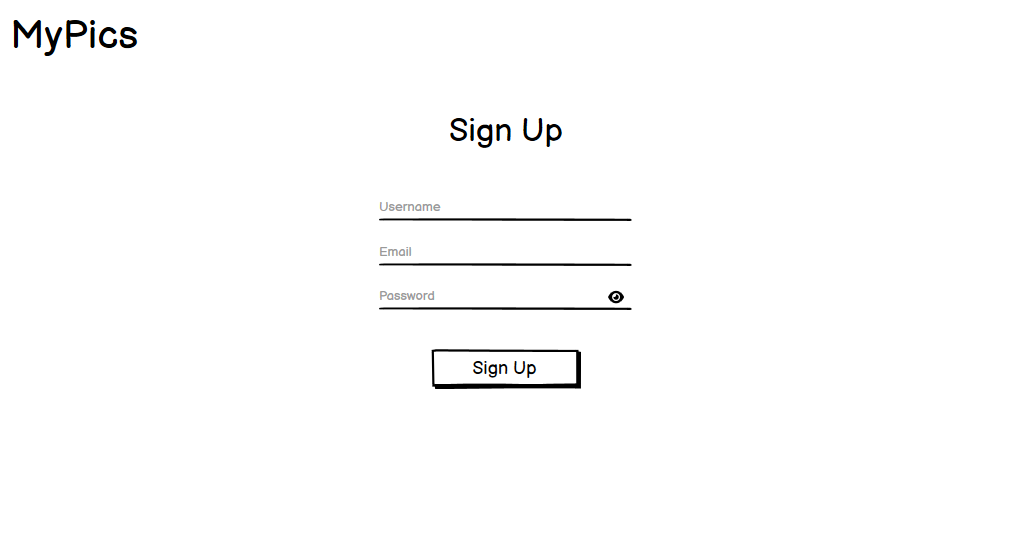
\includegraphics[width=0.6\textwidth]{images/sign-up.png}}
    %\caption{Caption}
    %\label{fig:my_label}
\end{figure}

\subsection{Login}
\begin{table}[H]
    \centering
    \begin{tabular}{|p{4.5cm}|p{4cm}|p{4cm}|p{4cm}|}
    \hline
    \rowcolor[HTML]{EFEFEF} 
    AS A                       & I WANT TO             & SO THAT I CAN         & ADDED BY \\ \hline
    Non-logged registered user & Login into the system & Use system's services & Everyone \\ \hline
    \end{tabular}
\end{table}
\begin{figure}[H]
    \centering
    \fbox{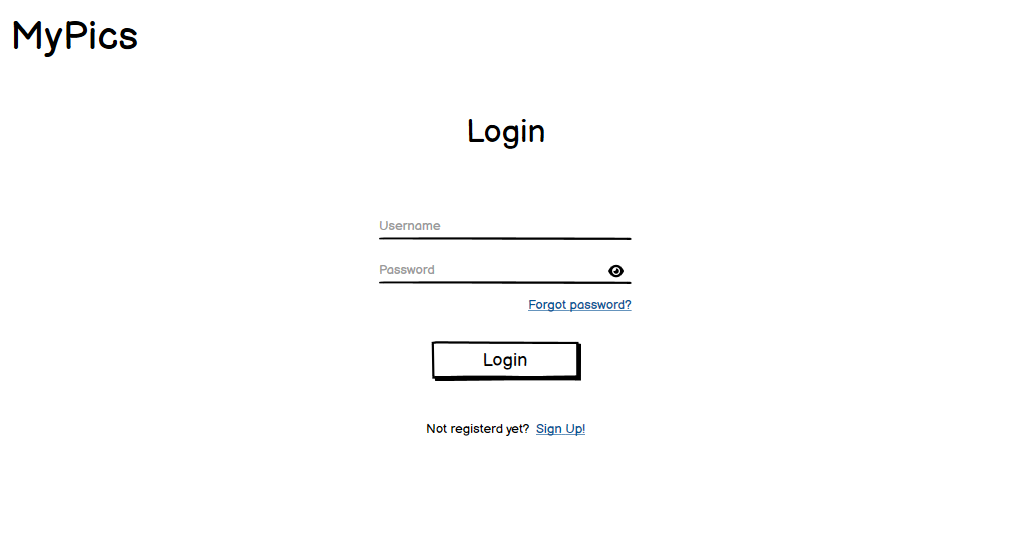
\includegraphics[width=0.6\textwidth]{images/login.png}}
    %\caption{Caption}
    %\label{fig:my_label}
\end{figure}

\subsection{Logout}
\begin{table}[H]
    \centering
    \begin{tabular}{|p{4.5cm}|p{4cm}|p{4cm}|p{4cm}|}
    \hline
    \rowcolor[HTML]{EFEFEF} 
    AS A                   & I WANT TO              & SO THAT I CAN & ADDED BY \\ \hline
    Logged registered user & Logout from the system &               & Everyone \\ \hline
    \end{tabular}
\end{table}
\begin{figure}[H]
    \centering
    \fbox{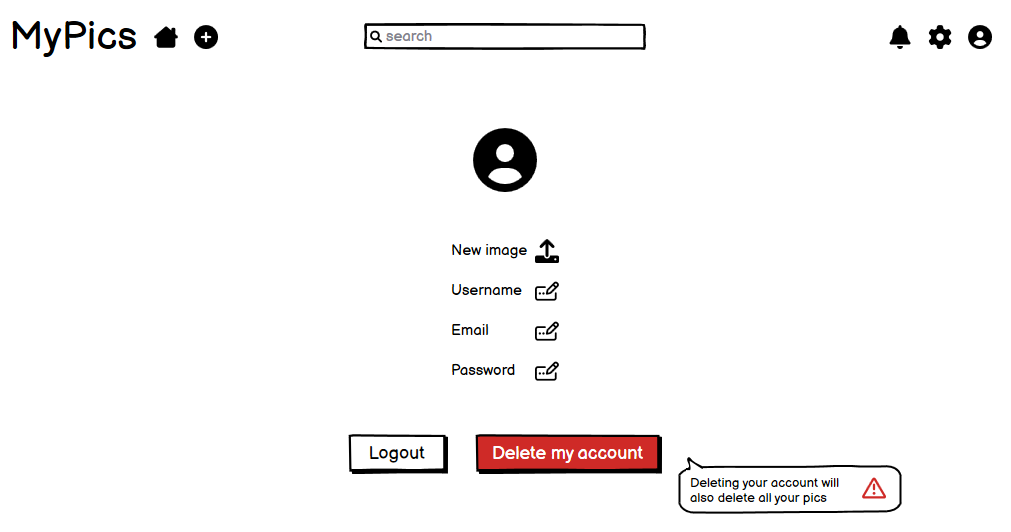
\includegraphics[width=0.6\textwidth]{images/settings.png}}
    %\caption{Caption}
    %\label{fig:my_label}
\end{figure}

\subsection{Main}
\begin{table}[H]
    \centering
    \begin{tabular}{|p{4.5cm}|p{4cm}|p{5cm}|p{3cm}|}
    \hline
    \rowcolor[HTML]{EFEFEF} 
    AS A            & I WANT TO                        & SO THAT I CAN                              & ADDED BY \\ \hline
    Registered user & Access the homepage              & Discover the most popular images           & Everyone \\ \hline
    Registered user & Search for images                & Visualize them                             & Everyone \\ \hline
    Registered user & Search for other users           & Visualize their profile and their images   & Everyone \\ \hline
    Registered user & Get notified                     & Know if another user liked one of my image & Everyone \\ \hline
    Registered user & Access my profile page           & Manage it                                  & Everyone \\ \hline
    Registered user & Access other user's profile page & Visualize his details and published images & Everyone \\ \hline
    \end{tabular}
\end{table}
\begin{figure}[H]
    \centering
    \fbox{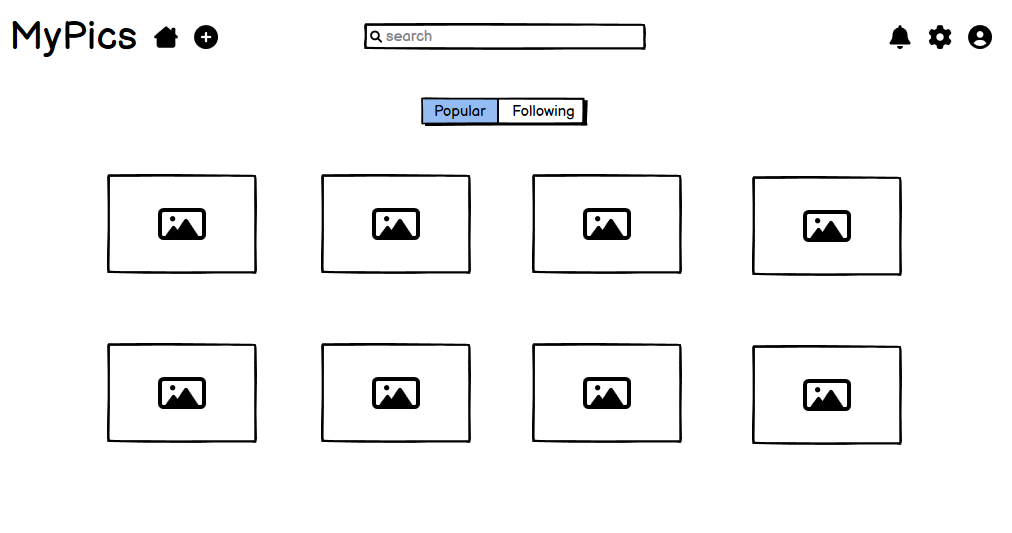
\includegraphics[width=0.6\textwidth]{images/home.png}}
    %\caption{Caption}
    %\label{fig:my_label}
\end{figure}

\subsection{Pic}
\begin{table}[H]
    \centering
    \begin{tabular}{|p{4.5cm}|p{4cm}|p{5cm}|p{3cm}|}
    \hline
    \rowcolor[HTML]{EFEFEF} 
    AS A            & I WANT TO                & SO THAT I CAN                       & ADDED BY \\ \hline
    Registered user & Like an image            & Express my appreciation about it    & Everyone \\ \hline
    Registered user & Save an image            & Discover the most popular images    & Everyone \\ \hline
    Registered user & Remove an uploaded image & Deny to other users to visualize it & Everyone \\ \hline    
    \end{tabular}
\end{table}
\begin{figure}[H]
    \centering
    \fbox{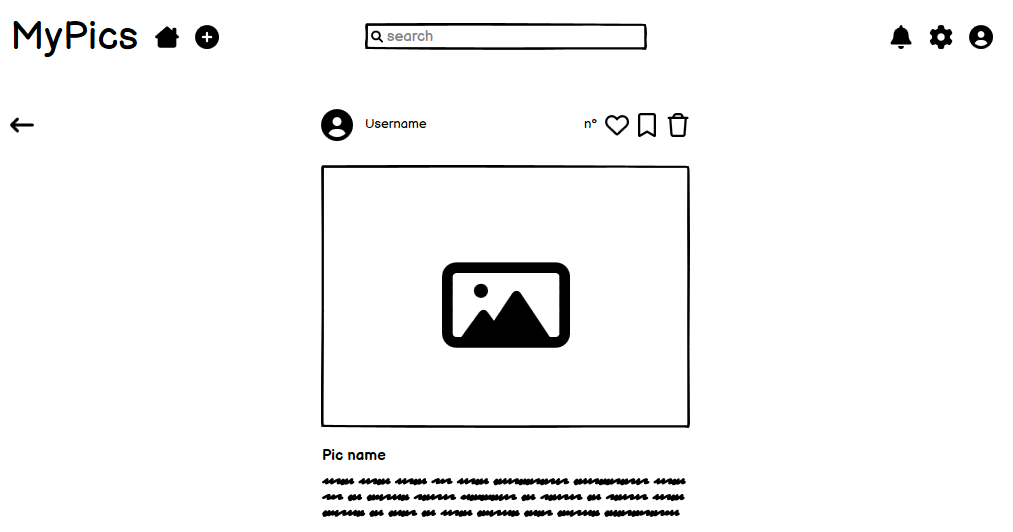
\includegraphics[width=0.6\textwidth]{images/pic.png}}
    %\caption{Caption}
    %\label{fig:my_label}
\end{figure}

\subsection{Upload pic}
\begin{table}[H]
    \centering
    \begin{tabular}{|p{4.5cm}|p{4cm}|p{5cm}|p{3cm}|}
    \hline
    \rowcolor[HTML]{EFEFEF} 
    AS A            & I WANT TO       & SO THAT I CAN             & ADDED BY \\ \hline
    Registered user & Upload an image & Share it with other users & Everyone \\ \hline    
    \end{tabular}
\end{table}
\begin{figure}[H]
    \centering
    \fbox{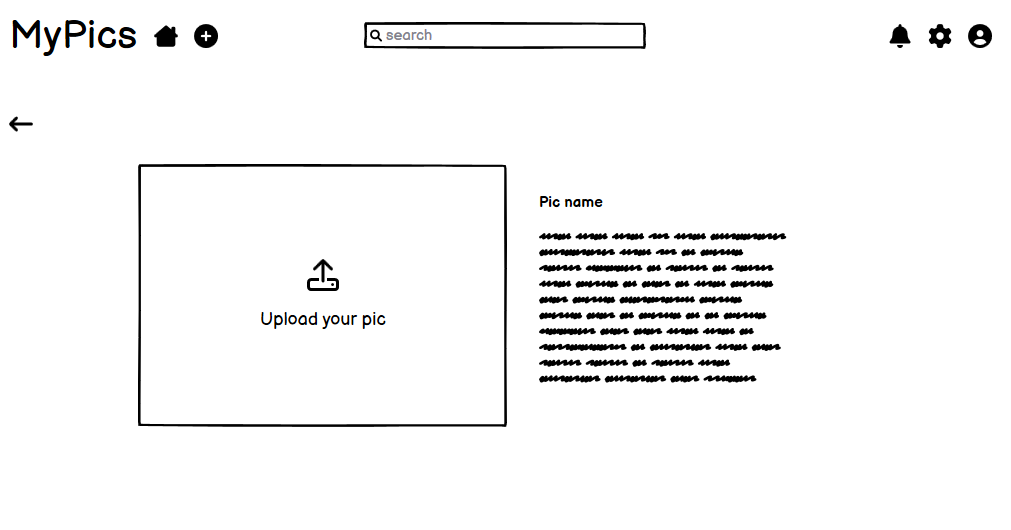
\includegraphics[width=0.6\textwidth]{images/addPic.png}}
    %\caption{Caption}
    %\label{fig:my_label}
\end{figure}

\subsection{User profile}
\begin{figure}[H]
    \centering
    \fbox{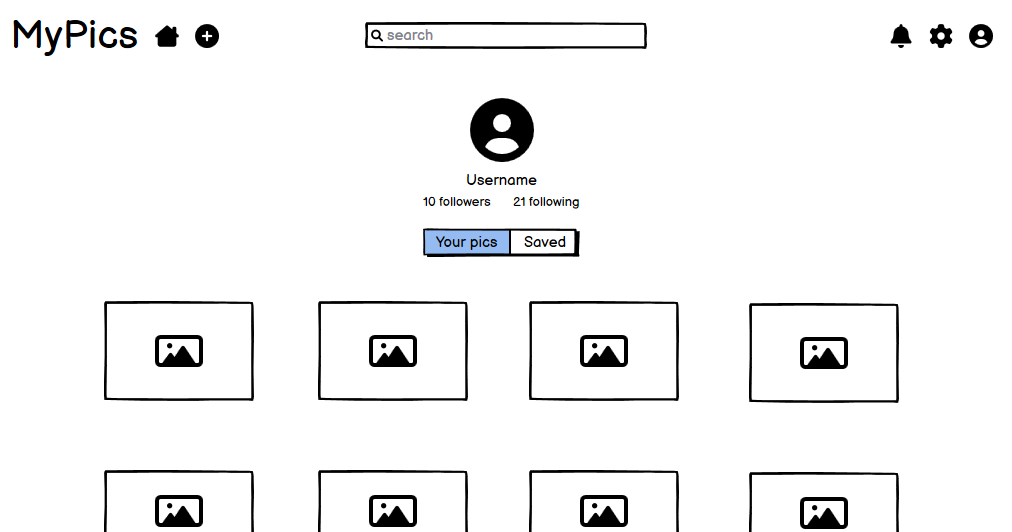
\includegraphics[width=0.45\textwidth]{images/profile.png}}
    \fbox{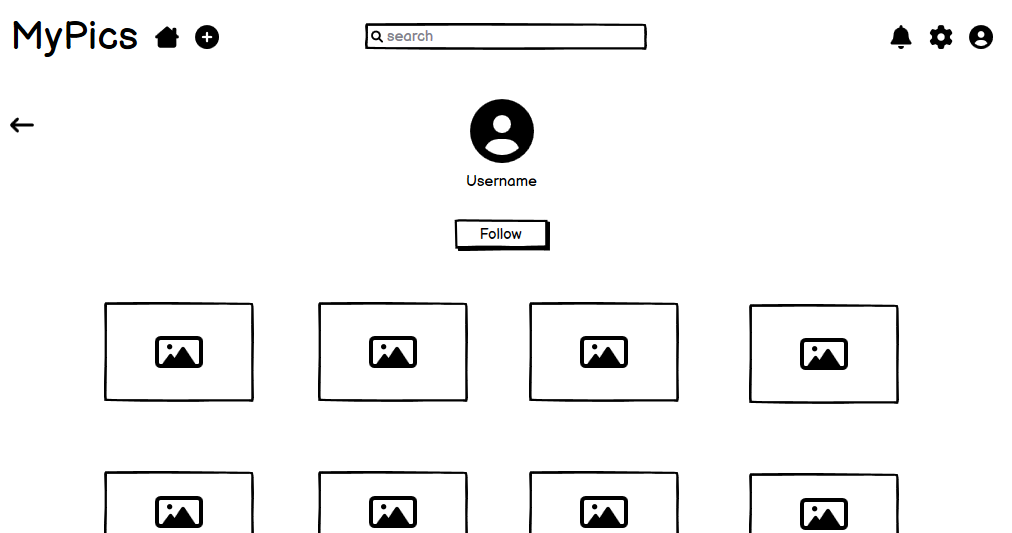
\includegraphics[width=0.45\textwidth]{images/user.png}}
    %\caption{Caption}
    %\label{fig:my_label}
\end{figure}

% Effort estimation ----------------------------------------------------------------

\newpage

\section{Effort estimation}

% System architecture ---------------------------------------------------------------

\newpage

\section{System architecture}

% Sprint analytics --------------------------------------------------------------------

\newpage

\section{Sprint analytics}


\end{document}
